\begin{scanpage}{0226}{208}
\begin{center}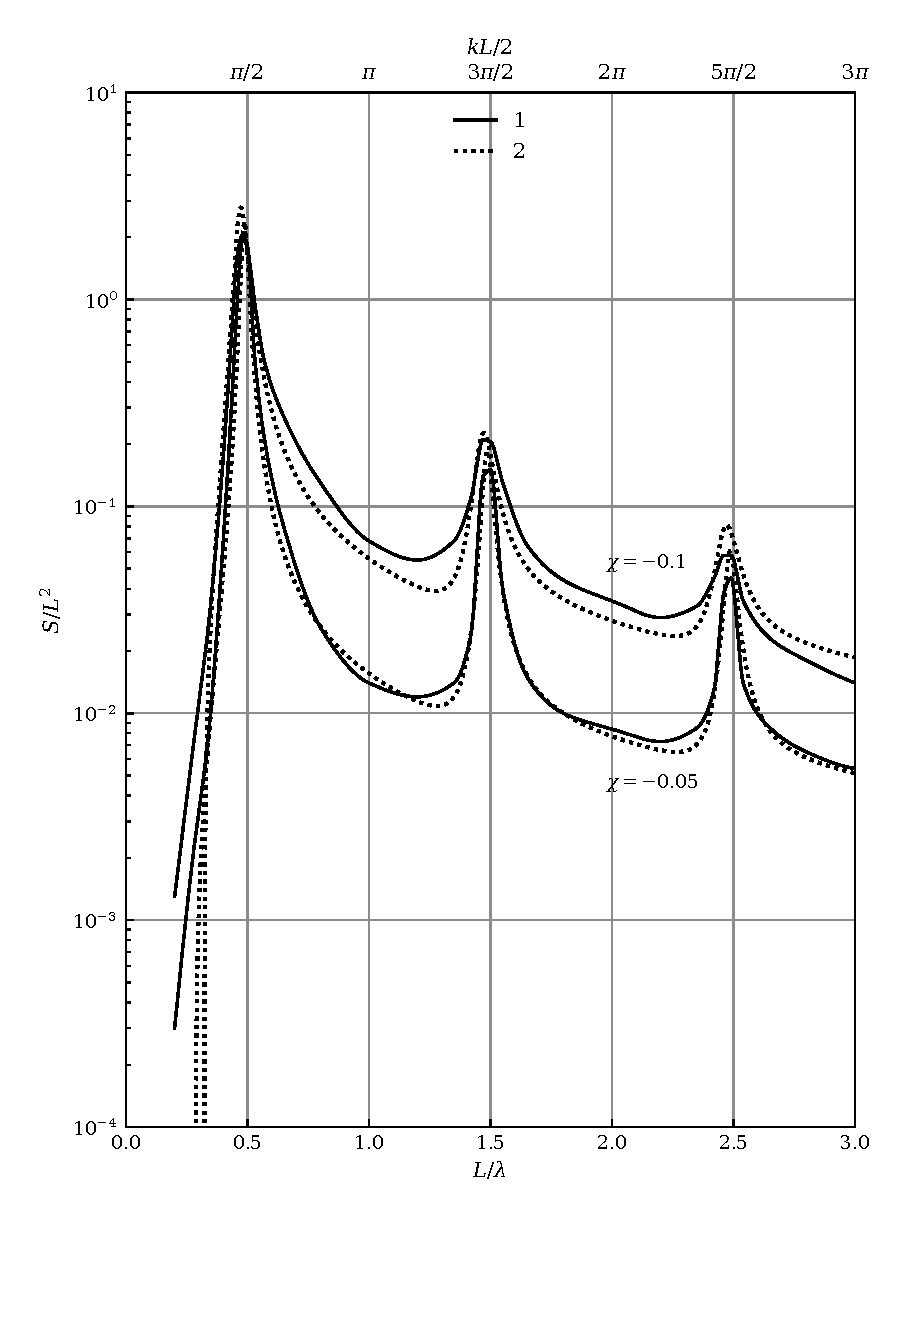
\includegraphics[width=.50\linewidth]{images/recreated/r-0226-fig76.pdf}\par
\begin{minipage}{.77\linewidth}Figure 76. The integral scattering thickness of a vibrator as a function of its length (with normal incidence of a plane wave). Curves 1 were calculated by Leontovich and Levin [85]. Curves 2 were calculated on the basis of Equation (34.07).\end{minipage}\end{center}
\[p_r=\frac{c}{8\pi}|E_\vartheta|^2=\frac{c}{8\pi}\frac{|F(\vartheta,\vartheta_0)|^2}{k^2R^2}E^2\tag{34.09}\]
represents the average value of the energy flux density scattered by the vibrator in the direction $\vartheta$. Consequently
\[\sigma(\vartheta,\vartheta_0)=\frac{\lambda^2}\pi\cos^2\alpha\cdot|F(\vartheta,\vartheta_0)|^2.\tag{34.10}\]
\end{scanpage}
